\chapter{Utilizing Spatial Sparsity}

For all but the smallest molecules, spatial sparsity is very important for achieving computational savings
in quantum chemistry. There exists two primary forms of spatial sparsity in (1.6). The first form
results from the Gaussian product $\mu(\textbf{r}_{1}) \nu(\textbf{r}_{1})$ diminishing with the overlap of the 
two AO Gaussians. This product diminishes rapidly with distance between the Gaussian function centers and is also 
highly sensitive to their degree of locality.
If the overlap between two AO Gaussians is insignificant, then it becomes unnecessary to compute any shell triplet featuring
this AO Gaussian pair.
Utilizing this pairwise sparsity requires only an estimation of the significant AO Gaussian pairs.
Once this spatial sparsity is applied and insignificant AO function pairs are screened, the complexity of 
computing the 3-center integrals becomes $\mathcal{O}(N_{aux}N_{AO}^{1-2})$, where the lower bound is achieved for sufficiently 
sparse systems. Another type of spatial sparsity in (1.6) involves the auxiliary function, which is more complicated to 
take advantage of. see Ref. \cite{ref5}. In this thesis, I focus on the former, pairwise sparsity which is featured
in the product $\mu(\textbf{r}_{1}) \nu(\textbf{r}_{1})$. 
Utilizing this sparsity not only speeds up the computation of the three-index integrals, but stored in a sparse format,
then this sparsity can be utilized in later operations such as the fitting metric contraction and basis transformations.

\section{Sparsity Masks}

The pairwise sparsity available to the 3-center integrals can be determined via an estimation of significant AO function pairs.
An implementation will require a two dimensional sparsity mapping structure which keeps track of the significant pairs.
We refer to these structures as sparsity masks, which are $N_{AO}$ by $N_{AO}$ Boolean matrices denoted as $S_{\mu \nu}^b$. 
The superscript $b$ reminds the reader that the structure is of Boolean type.
The element $S_{\mu \nu}^b$ will be true if the product $\mu(r)\nu(r)$ is estimated to be significant 
and false otherwise.

For efficiency, it is common to compute batches of integrals in \textit{shell triples}: 
\begin{align} 
(M N | Q) = \{(\mu \nu|P), \mu \in M, \nu \in N, Q \in P\} 
\end{align} 

\noindent An individual integral $(\mu \nu | P)$ is bounded by the Schwarz inequality $(\mu \nu | P) \leq 
\sqrt{(\mu \nu | \mu \nu)(P|P)}$. We can eliminate entire shells of integrals , $(MN|P)$, where $M$ and $N$ denote AO shells, by computing
and storing the maximum $(\mu \nu | \mu \nu)$ that occurs for a given shell $\mu \in M, \nu \in N$. We use a relative cutoff tolerance
$\tau$ and neglect shells for which 
\begin{align}
MN_{max} < \frac{\tau^2}{(\mu \nu | \mu \nu)_{max}},
\end{align}

\noindent where $MN_{max}$ is the maximum $(\mu \nu | \mu \nu)$
within a shell pair $(M, N)$ and $(\mu \nu | \mu \nu)_{max}$ is the global maximum $(\mu \nu | \mu \nu)$. In addition, even for shell pairs
that are not screened out, we can apply function-level screening and avoid computation of $(\mu \nu | P)$, where
\begin{align}
(\mu \nu | \mu \nu) < \frac{\tau^2}{(\mu \nu | \mu \nu)_{max}}.
\end{align}

Using this strategy, a sparsity mask can be easily constructed. Figure 2.1 includes
illustrations of sparsity masks for benzene stacks with 1, 5, and 10 benzenes spaced 3\text{\AA} apart. As sparsity increases, the number of
significant AO function pairs contained in these masks becomes $\mathcal{O}(N_{AO}^{1-2})$, where the lower bound is obtained for 
sufficiently sparse systems. 

\begin{figure}[H] 
\centering
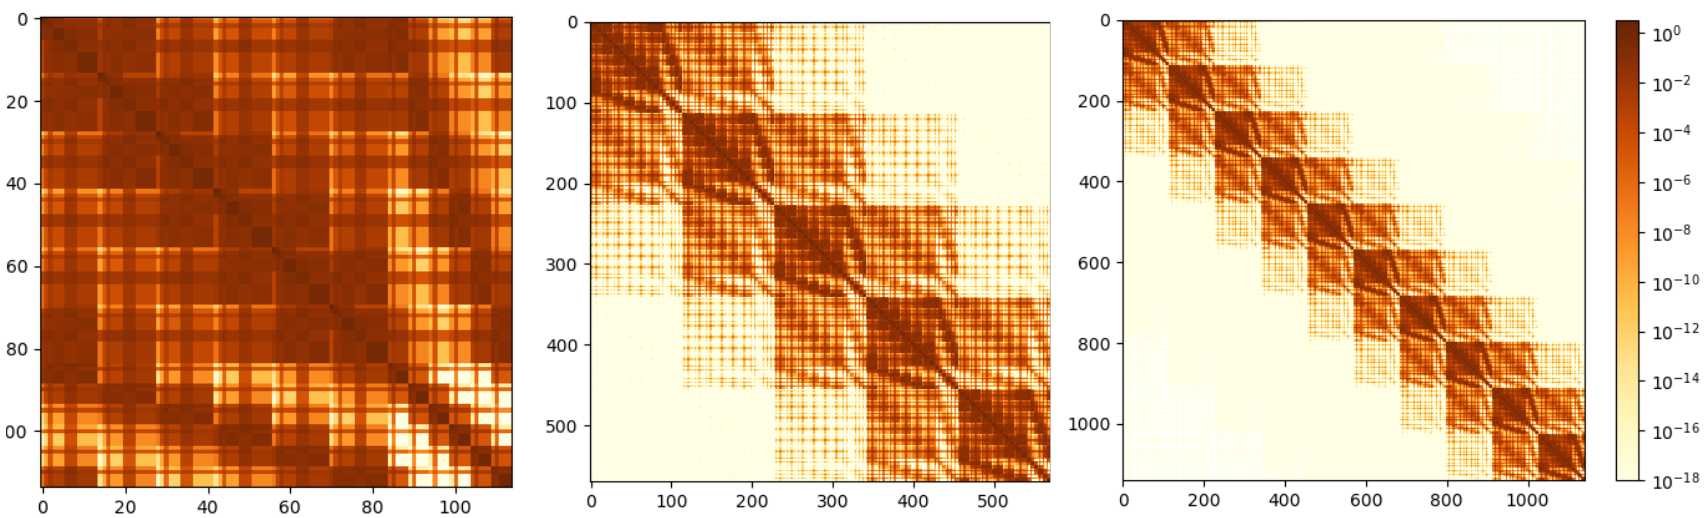
\includegraphics[scale=0.2]{figures/sparsity_plots/sparsity_masks.png} \caption{Schwarz sparsity masks used for benzene stacks containing 
1, 5, and 10 benzenes spaced 3\text{\AA}  apart. Sparsity masks were obtained by evaluating $(\mu\nu|\mu\nu)<\frac{\tau^2}{(\mu\nu|\mu\nu)_{max}}$.}
\label{fig:databases} \end{figure}


\section{Integral Construction}

Now, we are equipped to discuss the resulting algorithms when applying the integral sparsity to important operations such as
integral construction and transformation. To write more readable algorithms, 
we employ some tensor notation and write $A_{\mu \nu}^P$ to represent
the pre-contracted 3-center integrals $(\mu \nu |P)$. To prune these integrals using sparsity, 
the following algorithm can be employed:

\begin{algorithm}
\caption{Prune $A_{\mu \nu}^P$ using sparsity}
\begin{algorithmic}
\REQUIRE AO integrals: $A_{\mu \nu}^P$, screening mask: $S_{\mu \nu}^b$
\FOR {$\mu = 0$ to $\mu = N_{AO}-1$}  
    \STATE $A_{\mu \nu}^P S_{\mu \nu}^b \rightarrow A_{\mu \nu^{\mu}}^P$
\ENDFOR
\RETURN $A_{\mu \nu^\mu}^P$
\end{algorithmic}
\end{algorithm}

\noindent Here we have introduced the symbol $\nu^\mu$, which indicates that $\nu$ is restricted to AO functions
which are spatially close enough to $\mu$ to survive the Schwarz screening process. The superscript in $\nu^\mu$ 
indicates a dependence of $\nu$ according to $\mu$. Algorithm 1 is purely pedagogical, as one would never
build the full $A_{\mu \nu}^P$ integrals and then prune them for sparsity. 
Rather, sparsity screening would be applied as the integrals are constructed and insignificant
function triplets are never computed. The computation
and storage of $A_{\mu \nu^\mu}^P$ scales as $\mathcal{O}(N_{aux}N_{AO}^{1-2})$. 
Moreover, the costly metric contraction becomes
\begin{align} 
B_{\mu \nu^\mu}^Q = A_{\mu \nu^\mu}^P[J]_{PQ}^{-\frac{1}{2}}
\end{align}
\noindent and scales as $\mathcal{O}(N_{aux}^2N_{AO}^{1-2})$, where the lower bound is achieved for sufficiently sparse
systems.

\section{Integral Transformation}

The transformation of $A_{\mu \nu}^P$ (or $B_{\mu \nu^\nu}^Q$) from the AO basis to the MO basis is 
an essential operation for many quantum 
chemistry procedures. The operation requires two MO matrices: $C_{\mu p}, C_{\nu q}$, where $p, q$ are general MO space
indices. A first contraction $A_{p \nu}^P=A_{\mu \nu}^PC_{\mu p}$ will half-transform the integrals and costs 
$\mathcal{O}(N_{aux}N_{AO}^2N_p)$. The second contraction $A_{p q}^P=A_{p \nu}^PC_{\nu q}$ will cost
$\mathcal{O}(N_{aux}N_{AO}N_pN_q)$.
Note the first contraction should involve the smaller of $N_p$ and $N_q$ in order to reduce complexity. Also, the first contraction
is comparably more expensive than the latter since the size of the AO space is larger than most MO spaces. Therefore,
reducing the cost of the first contraction would alleviate a bottleneck overall. 
Thankfully, we can exploit the sparsity of $A_{\mu \nu^\mu}^P$.
To do so, we carry out a looping DGEMM through the $\mu$ index and apply the sparsity mask to the orbital matrix $C_{\mu p}$.
Algorithm 2 illustrates the resulting process:

\begin{algorithm}[H]
\caption{Transform sparse integrals $A_{\mu \nu^\mu}^P$ to MO spaces.}
\begin{algorithmic}
\REQUIRE Sparse AO integrals: $A_{\mu \nu^\mu}^P$, orbital matrices: $C_{\mu p}, C_{\nu q}$, screening mask: $S_{\mu \nu}^b$
\FOR {$\mu = 0$ to $\mu = N_{AO}-1$}  
    \STATE $C_{\nu q}S_{\mu \nu}^b \rightarrow C_{\nu^{\mu} q}$
    \STATE $A_{\mu \nu^{\mu}}^P C_{\nu^{\mu} q} \rightarrow A_{\mu q}^P$
\ENDFOR
\STATE $A_{\mu q}^PC_{\mu p} \rightarrow A_{p q}$
\RETURN $A_{p q}^P$
\end{algorithmic}
\end{algorithm}


\section{Results}

All methods were implemented in the {\sc Psi4} electronic structure software package.
The parallelism in {\sc Psi4} relies on the shared memory programming model using OpenMP 
and carries out matrix multiplications using Intel's Math Kernel
Library. 

We demonstrate the performance of our Schwarz screening implementation 
by measuring the performance when computing the 3-center integrals, contracting the fitting metric,
and transforming the integrals into an MO basis.
The experiment employed an ideal sparse system: stacked benzenes. Execution times were recorded for each successive benzene
added to the stack, from one to ten benzenes, with each benzene spaced 5\AA\ apart.
Transformation time involved the wall time required to carry out the common occupied-virtual
transformation, as would be required by density-fitted MP2: 
\begin{align} 
(i b | Q) = (\lambda \sigma | Q) C_{\sigma i} C_{\lambda b} 
\end{align}

\noindent Where $i, j$ and $a, b$ denote occupied and virtual spaces, respectively. 
Algorithm 4 was implemented and used to carry out these transformations.
The cc-pVTZ and cc-pVTZ-jkfit basis sets were used for primary 
and auxiliary basis sets, respectively. The characteristics
of each system are listed in Table 2.1. The mask sparsity listed in Table 2.1 refers to the percentage of non-significant AO function pairs appearing in the sparsity mask.
The experiment was carried out using one node consisting of an Intel Core i7-5930K processor 
(6 cores at 3.50GHz) and 50GB DRAM. The results are plotted in Figure 2.2. Figure 2.2 (a), (b), (c), and (d) involve time to compute the 3-index integrals, contract the fitting metric,
perform the first transformation step: $(\mu \nu | Q)C_{i \mu} \rightarrow (i \nu | Q)$,
and total transform time, respectively.
Note that our novel contribution involves the application of the sparsity screening in the transformation step.

\begingroup
\begin{table}[H]
\centering
\renewcommand{\baselinestretch}{1}
\caption{Characteristics of benzene stack systems. $N$ and $N_{aux}$ refer to the number of primary and auxiliary basis functions, respectively.
 Mask sparsity refers to the percentage of significant AO function pairs in the sparsity mask. Mask sparsity increases with additional benzenes added to the stack.}
\begin{tabular}{l ccc}
\multicolumn{1}{l}{\textbf{Benzenes}} &
\multicolumn{1}{c}{\textbf{$N$}} &
\multicolumn{1}{c}{\textbf{$N_{aux}$}} &
\multicolumn{1}{c}{\textbf{Mask Sparsity (\%)}} \\
\hline
1        & 264  & 654       & 2.6              \\ 
2        & 528  & 1308      & 24.7             \\ 
3        & 792  & 1962      & 43.6             \\ 
4        & 1056 & 2616      & 55.3             \\ 
5        & 1320 & 3270      & 63.1             \\ 
6        & 1584 & 3924      & 68.6             \\ 
7        & 1848 & 4578      & 72.7             \\ 
8        & 2112 & 5232      & 75.9             \\ 
9        & 2376 & 5886      & 78.4             \\ 
10       & 2640 & 6540      & 80.4             \\ 
\end{tabular}
\end{table}
\endgroup

\begin{figure}[H]
  \centering
  \subfloat[]{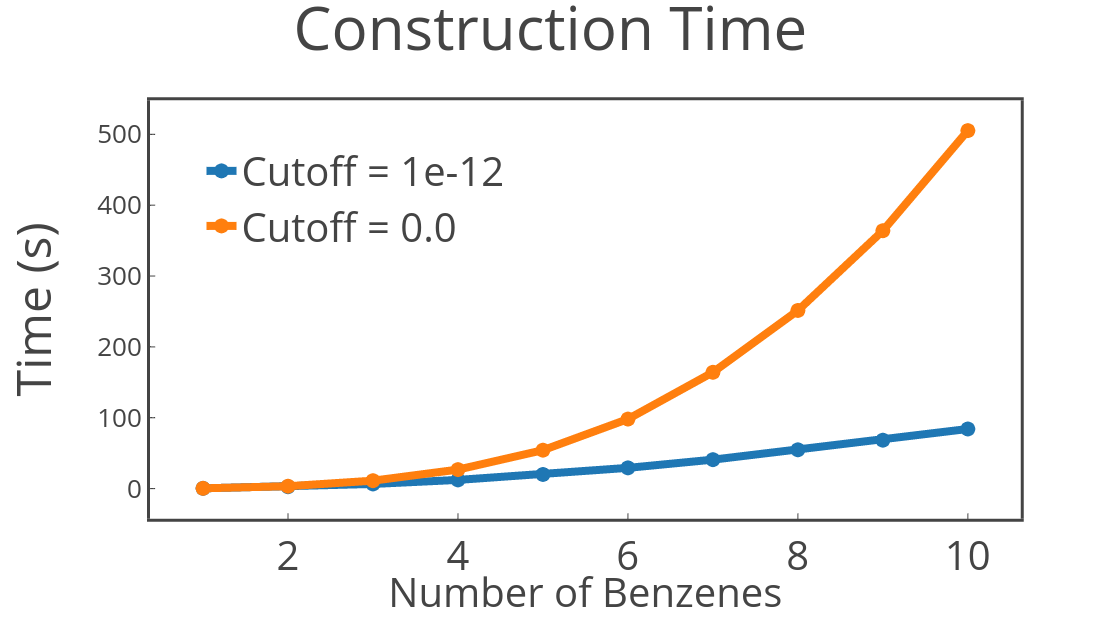
\includegraphics[width=0.5\textwidth]{figures/sparsity_plots/construction_wall.png}\label{fig:f1}}
  \hfill
  \subfloat[]{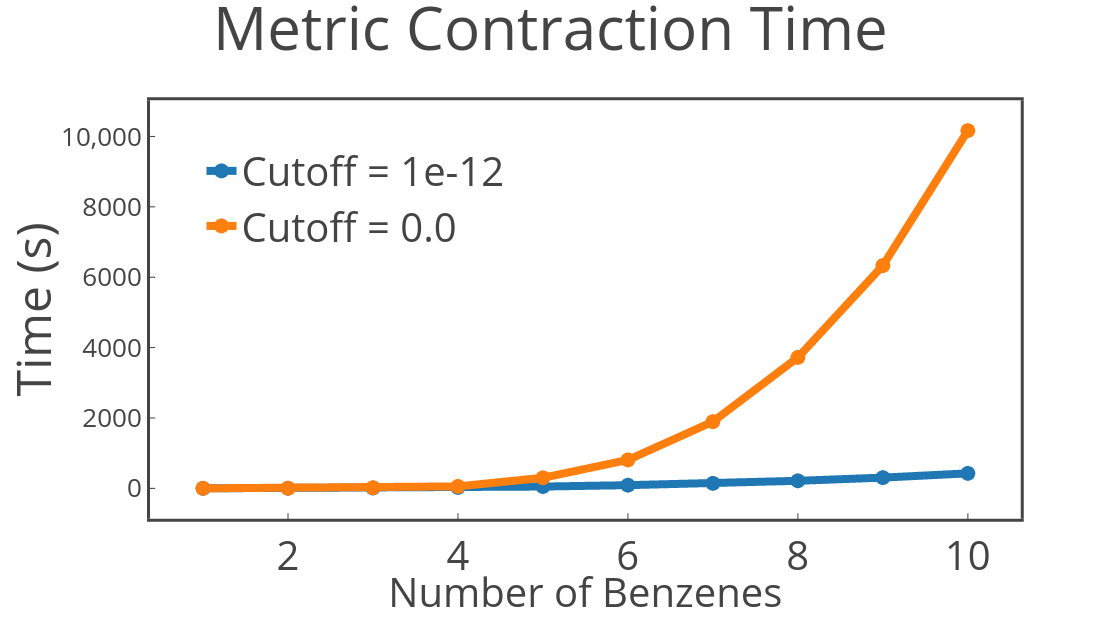
\includegraphics[width=0.5\textwidth]{figures/sparsity_plots/metric_contraction.png}\label{fig:f1}}
  \hfill \\
  \subfloat[]{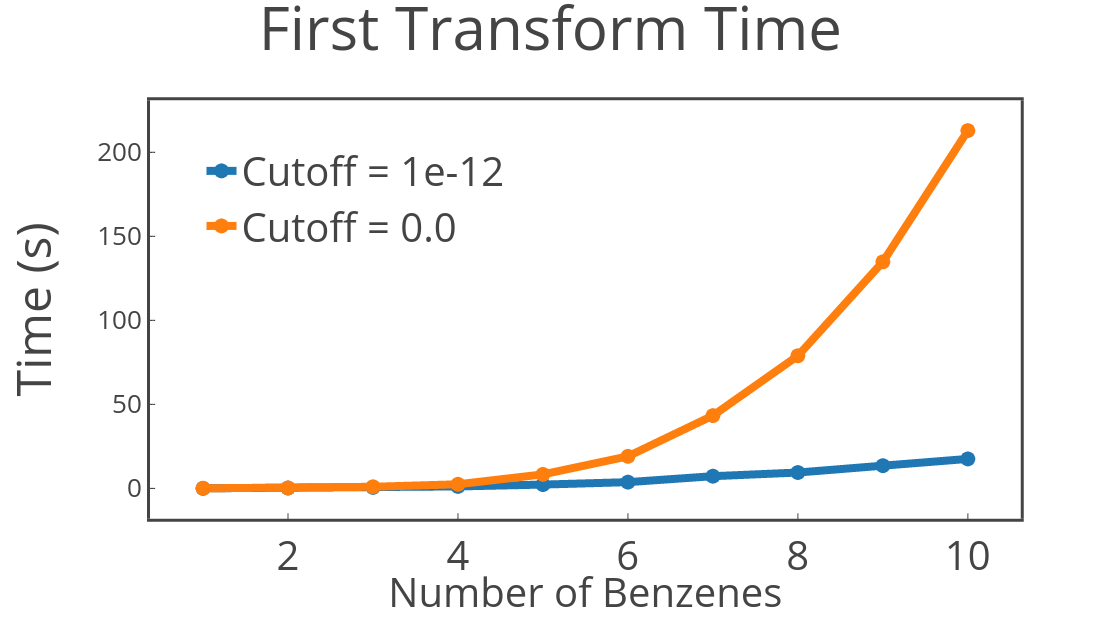
\includegraphics[width=0.5\textwidth]{figures/sparsity_plots/first_transform_wall.png}\label{fig:f1}}
  \hfill
  \subfloat[]{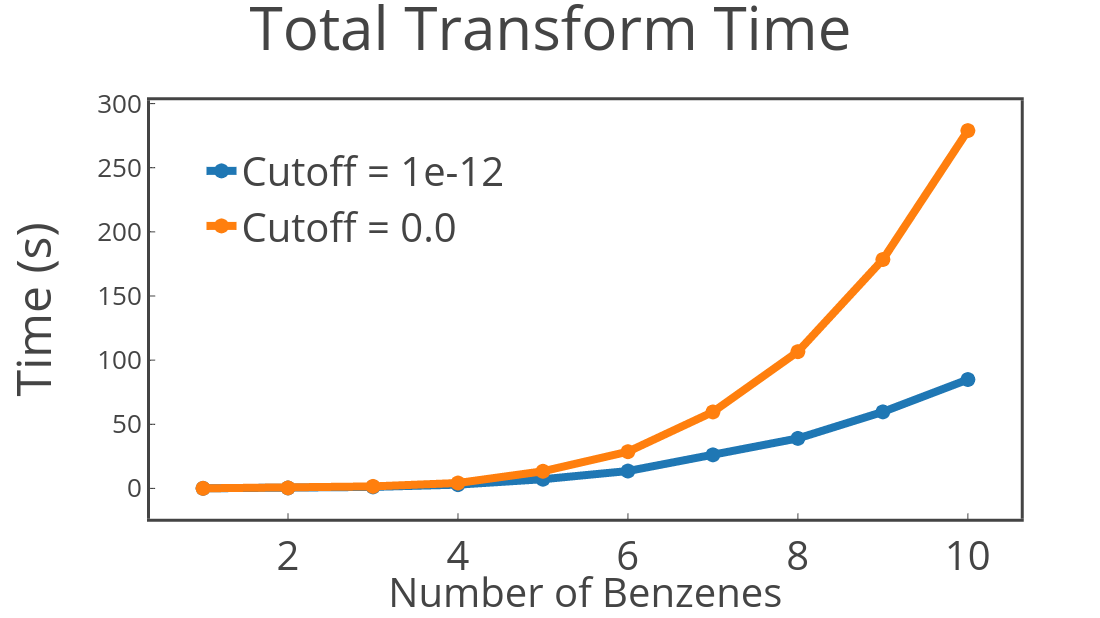
\includegraphics[width=0.5\textwidth]{figures/sparsity_plots/total_transform_wall.png}\label{fig:f2}}
  \caption{Comparison of execution times using sparsity screening (blue) against no sparsity screening (orange). Execution time is plotted against number of benzenes
 in a benzene stack from one to ten benzenes. Transformations involved computing $(ib|Q)$, where $i$ and $b$ denote occupied and virtual indices, respectively.
 Cutoff refers to the Schwarz screening threshold. (a) Computing the integrals. (b) Contracting AO integrals with the fitting metric. 
(c) First transformation times only. (d) Sum of first and second transformation times.}
\end{figure}

\noindent The cost of the first contraction becomes $\mathcal{O}(N_{aux}N_{AO}^{1-2}N_p)$. 
The remaining sparsity in the half-transformed $A_{\nu q}^P$ is unrelated to the original sparsity mask.

\begingroup
\begin{table}[H]
\centering
\renewcommand{\baselinestretch}{1}
\caption{Speedups obtained from sparsity screening at ten benzenes from data in Figure 2.2.}
\begin{tabular}{l c}
\multicolumn{1}{l}{\textbf{Operation}} &
\multicolumn{1}{c}{\textbf{Speedup at 10 benzenes}} \\ 
\hline
Construction          & 10.6  \\          
Metric Contraction    & 37.8  \\          
First Transformation  & 25.8  \\          
Total Transformation  & 5.5  \\          
\end{tabular}
\end{table}
\endgroup


Clearly, Figure 2.2 reveals significant time reductions for all procedures measured.
Table 2.2 reinforces that operations with higher complexity scaling have the largest time
reduction, with the caveat that total transformation time includes portions without sparsity utilization.
In the integral computations (Figure 2.2 (a)), we construct the sparse integrals using
function screening; however, we still compute them in shell triplets for efficiency.
Therefore the acquired speedup is slightly less dramatic compared to the metric contraction and
transformation procedures (Figure 2.2 (b) and (c), respectively) due to select functions being 
screened in cases where the entire shell is not screened. 
Note that the metric contraction is by far the most expensive operation, which should in one part
highlight the boon of sparsity utilization and in another part
illustrate the pertinence of our workflow investigation in Chapter 3 of this thesis.
Last, our proposal outlined in Algorithm 2 for applying sparsity screening to integral transformations
is proven viable by Figure 2.2 (c). Note that significant reductions are obtained for the
first transformation; however, the sparsity thereafter is unrelated to the initial sparsity
mask. With sparsity utilization, the first step scales as $\mathcal{O}(N_{aux}N_{AO}^{1-2}p)$,
whereas the second transformation step will still scale as $\mathcal{O}(N_{aux}N_pN_q)$.
In this work we have not gone on to consider sparsity of the MO indices, which would 
typically require transformation to local orbitals.


